%!TEX program = xelatex
%!TEX root = ../all_beamer.tex


%% Nonparametric Classification – Beamer Presentation
%% Based on notes by Giorgio Gambosi, University of Rome "Tor Vergata"
%% Style modelled on ml-linclass-beamer.tex

%% !TEX root = all_beamer.tex
% ==============================================================================
% HEADER LATEX PER PRESENTAZIONI BEAMER
% Corso di Machine Learning - Giorgio Gambosi
% Università di Roma "Tor Vergata"
% ==============================================================================

% ------------------------------------------------------------------------------
% CLASSE DOCUMENTO E METADATI
% ------------------------------------------------------------------------------
\documentclass[aspectratio=169, 10pt]{beamer}

\subtitle{Course of Machine Learning}
\author{Giorgio Gambosi}
\institute[Tor Vergata]{Master's Degree in Computer Science\\University of Rome ``Tor Vergata''}
\date{A.Y. 2025--2026}

% ------------------------------------------------------------------------------
% PACCHETTI MATEMATICI
% ------------------------------------------------------------------------------
\usepackage{amsmath, amssymb, amsfonts, mathtools, amsthm}
\usepackage{bm}              % Simboli matematici in grassetto
\usepackage{upgreek}         % Lettere greche dritte
\usepackage{derivative}      % Gestione semplificata delle derivate

% ------------------------------------------------------------------------------
% PACCHETTI GRAFICI E VISUALIZZAZIONE
% ------------------------------------------------------------------------------
\usepackage{graphicx}        % Inclusione immagini
\usepackage{xcolor}          % Gestione colori
\usepackage{xkcdcolors}      % Colori aggiuntivi stile xkcd
\usepackage{microtype}       % Miglioramenti tipografici

% ------------------------------------------------------------------------------
% PACCHETTI PER TABELLE
% ------------------------------------------------------------------------------
\usepackage{booktabs}        % Tabelle professionali
\usepackage{array}           % Estensioni per tabelle
\usepackage{multirow}        % Celle multi-riga
\usepackage{multicol}        % Layout multi-colonna

% ------------------------------------------------------------------------------
% TIKZ E PGFPLOTS
% ------------------------------------------------------------------------------
\usepackage{tikz}
\usepackage{tikz-network}
\usepackage[customcolors]{hf-tikz}
\usepackage{pgfplots}
\pgfplotsset{compat=1.18}
\usepgfplotslibrary{fillbetween}

% Librerie TikZ
\usetikzlibrary{arrows, arrows.meta, decorations.pathmorphing, decorations.pathreplacing}
\usetikzlibrary{decorations.markings, snakes, positioning, backgrounds, fit, shadows}
\usetikzlibrary{automata, patterns, calc, intersections, through, shapes}
\usetikzlibrary{shapes.geometric, shapes.arrows, scopes, chains, matrix}

% ------------------------------------------------------------------------------
% ALTRI PACCHETTI
% ------------------------------------------------------------------------------
\usepackage[skins]{tcolorbox}  % Box colorati
\usepackage{subcaption}         % Sottocaption per figure
\usepackage{listings}           % Inclusione codice sorgente

% ------------------------------------------------------------------------------
% TEMA E STILE BEAMER
% ------------------------------------------------------------------------------
\usetheme{Madrid}
\usecolortheme{whale}
\useinnertheme{rounded}
\usefonttheme{professionalfonts}
\setbeamertemplate{navigation symbols}{}  % Rimuove simboli di navigazione

% ------------------------------------------------------------------------------
% DEFINIZIONE COLORI PERSONALIZZATI
% ------------------------------------------------------------------------------
% Colori principali del tema
\definecolor{MainBlue}{RGB}{31,56,100}      % Blu principale (header, titoli)
\definecolor{AccentBlue}{RGB}{70,130,180}   % Blu accento (blocchi)
\definecolor{AlertRed}{RGB}{160,30,30}      % Rosso per alert
\definecolor{ExGreen}{RGB}{30,120,60}       % Verde per esempi
\definecolor{BlockBg}{RGB}{220,232,246}     % Sfondo blocchi
\definecolor{torgray}{RGB}{220,225,235}     % Grigio Tor Vergata

% Colori alternativi (Tor Vergata style)
\definecolor{TvDark}{RGB}{30,50,80}         % Blu scuro header
\definecolor{TvMid}{RGB}{70,100,140}        % Blu medio blocchi
\definecolor{TvLight}{RGB}{210,220,235}     % Blu chiaro sfondi
\definecolor{TvAlert}{RGB}{160,30,30}       % Rosso alert
\definecolor{TvGreen}{RGB}{20,100,50}       % Verde esempi

% Colori supplementari
\definecolor{torred}{RGB}{153,0,0}
\definecolor{torcyan}{RGB}{0,112,192}
\definecolor{cerise}{HTML}{DA3A62}
\definecolor{teal}{HTML}{029386}
\definecolor{slateblue}{HTML}{5B5EA6}
\definecolor{orange}{HTML}{F97306}

% Colori per nodi TikZ
\definecolor{nodeblue}{RGB}{101,140,196}    % xkcd Faded Blue

% ------------------------------------------------------------------------------
% CONFIGURAZIONE COLORI BEAMER
% ------------------------------------------------------------------------------
\setbeamercolor{frametitle}{bg=MainBlue, fg=white}
\setbeamercolor{title}{bg=MainBlue, fg=white}
\setbeamercolor{structure}{fg=MainBlue}

% Blocchi standard
\setbeamercolor{block title}{bg=AccentBlue, fg=white}
\setbeamercolor{block body}{bg=BlockBg}

% Blocchi alert
\setbeamercolor{block title alerted}{bg=AlertRed, fg=white}
\setbeamercolor{block body alerted}{bg=red!8}

% Blocchi esempio
\setbeamercolor{block title example}{bg=ExGreen, fg=white}
\setbeamercolor{block body example}{bg=green!7}

% ------------------------------------------------------------------------------
% CONFIGURAZIONE FONT BEAMER
% ------------------------------------------------------------------------------
\setbeamerfont{frametitle}{size=\normalsize,series=\bfseries}
\setbeamerfont{block title}{size=\small,series=\bfseries}

% ------------------------------------------------------------------------------
% STILI TIKZ PERSONALIZZATI
% ------------------------------------------------------------------------------
\tikzset{
  >=latex,  % Frecce stile LaTeX di default
  % Nodi per reti neurali
  node/.style={thick,circle,draw=myblue,minimum size=22,inner sep=0.5,outer sep=0.6},
  node in/.style={node,green!20!black,draw=mygreen!30!black,fill=mygreen!25},
  node hidden/.style={node,blue!20!black,draw=myblue!30!black,fill=myblue!20},
  node convol/.style={node,orange!20!black,draw=myorange!30!black,fill=myorange!20},
  node out/.style={node,red!20!black,draw=myred!30!black,fill=myred!20},
  % Connessioni
  connect/.style={thick,mydarkblue},
  connect arrow/.style={-{Latex[length=4,width=3.5]},thick,mydarkblue,shorten <=0.5,shorten >=1},
  % Stili numerati per facile mappatura
  node 1/.style={node in},
  node 2/.style={node hidden},
  node 3/.style={node out}
}

% ------------------------------------------------------------------------------
% AMBIENTI TEOREMI
% ------------------------------------------------------------------------------
\setbeamertemplate{theorems}[numbered]
\newtheorem{mytheorem}{Theorem}
\newtheorem{mydefinition}{Definition}

% ------------------------------------------------------------------------------
% CONFIGURAZIONE LISTINGS (CODICE)
% ------------------------------------------------------------------------------
\lstset{
  language=Python,
  basicstyle=\ttfamily\tiny,
  keywordstyle=\color{MainBlue}\bfseries,
  commentstyle=\color{gray},
  frame=single,
  breaklines=true,
}

% ==============================================================================
% MACRO MATEMATICHE PERSONALIZZATE
% ==============================================================================

% ------------------------------------------------------------------------------
% SPAZI CALLIGRAFICI (Calligraphic spaces)
% ------------------------------------------------------------------------------
\providecommand{\calX}{\mathcal{X}}         % Spazio input
\providecommand{\calY}{\mathcal{Y}}         % Spazio output
\providecommand{\calH}{\mathcal{H}}         % Spazio ipotesi
\providecommand{\calT}{\mathcal{T}}         % Training set
\providecommand{\calA}{\mathcal{A}}         % Algoritmo
\providecommand{\calR}{\mathcal{R}}         % Rischio
\providecommand{\calF}{\mathcal{F}}         % Famiglia di funzioni
\providecommand{\calL}{\mathcal{L}}         % Loss function

% Alias per compatibilità
\providecommand{\Rr}{\mathcal{R}}
\providecommand{\Tr}{\mathcal{T}}
\providecommand{\Hr}{\mathcal{H}}

% ------------------------------------------------------------------------------
% RISCHIO E PROBABILITÀ
% ------------------------------------------------------------------------------
\providecommand{\barR}{\overline{\mathcal{R}}}  % Rischio empirico
\providecommand{\EmpR}{\overline{\mathcal{R}}}  % Rischio empirico (alias)
\providecommand{\Rbar}{\overline{\mathcal{R}}}  % Rischio empirico (alias)
\providecommand{\pM}{p_M}                       % Probabilità modello
\providecommand{\pC}{p_C}                       % Probabilità corretta
\providecommand{\Prob}[2]{\mathbb{P}_{#1}\!\left[#2\right]}  % Probabilità

% ------------------------------------------------------------------------------
% FUNZIONI INDICATRICI
% ------------------------------------------------------------------------------
\providecommand{\indicator}[1]{\mathbf{1}\!\left[#1\right]}  % Funzione indicatrice
\providecommand{\ind}[1]{\mathbf{1}[#1]}                      % Versione breve

% ------------------------------------------------------------------------------
% OPERATORI MATEMATICI
% ------------------------------------------------------------------------------
\providecommand{\argmax}{\operatorname*{arg\,max}}  % Argomento del massimo
\providecommand{\argmin}{\operatorname*{arg\,min}}  % Argomento del minimo
\providecommand{\vcd}[1]{\operatorname{VCdim}(#1)} % VC dimension
\providecommand{\defeq}{\stackrel{\text{def}}{=}}  % Definito come

% ------------------------------------------------------------------------------
% VETTORI E MATRICI (Bold Math)
% ------------------------------------------------------------------------------
% Vettori minuscoli
\providecommand{\bx}{\mathbf{x}}            % Vettore x
\providecommand{\bz}{\mathbf{z}}            % Vettore z
\providecommand{\bw}{\mathbf{w}}            % Vettore peso
\providecommand{\btt}{\mathbf{t}}           % Vettore target
\providecommand{\wvec}{\mathbf{w}}          % Vettore peso (alias)
\providecommand{\bth}{\boldsymbol{\theta}}  % Parametro theta

% Matrici maiuscole
\providecommand{\bX}{\mathbf{X}}            % Matrice dati
\providecommand{\bZ}{\mathbf{Z}}            % Matrice Z
\providecommand{\Xmat}{\mathbf{X}}          % Matrice dati (alias)
\providecommand{\Hmat}{\mathbf{H}}          % Matrice H
\providecommand{\Smat}{\mathbf{S}}          % Matrice scatter generica
\providecommand{\bS}{\mathbf{S}}            % Matrice scatter
\providecommand{\Ii}{\mathbf{I}}            % Matrice identità
\providecommand{\bZero}{\mathbf{0}}         % Vettore zero
\providecommand{\bPsi}{\boldsymbol{\Psi}}   % Matrice Psi

% Medie (overline)
\providecommand{\ox}{\overline{\mathbf{x}}} % Media vettore x
\providecommand{\ow}{\overline{\mathbf{w}}} % Media vettore w
\providecommand{\oX}{\overline{\mathbf{X}}} % Media matrice X

% Matrici scatter specifiche (analisi discriminante)
\providecommand{\SW}{\mathbf{S}_W}          % Within-class scatter
\providecommand{\SB}{\mathbf{S}_B}          % Between-class scatter
\providecommand{\ST}{\mathbf{S}_T}          % Total scatter
\providecommand{\GX}{G_{\mathbf{X}}}        % Matrice Gram

% ------------------------------------------------------------------------------
% COMANDI DI FORMATTAZIONE TESTO
% ------------------------------------------------------------------------------
\providecommand{\term}[1]{\textbf{\color{accent}#1}}        % Termine importante
\providecommand{\halert}[1]{{\color{AlertRed}\textbf{#1}}}  % Alert rosso
\providecommand{\mlalert}[1]{{\color{AccentBlue}\textbf{#1}}}  % Alert blu
\providecommand{\mlemph}[1]{{\color{MainBlue}\textit{#1}}}  % Enfasi blu

% ==============================================================================
% FINE HEADER
% ==============================================================================

\newcommand{\blankpage}{
\clearpage
\thispagestyle{empty}
\null
\clearpage
}

%
%%% ── Packages ────────────────────────────────────────────────────────────────
%\usepackage{amsmath,amssymb,bm}
%\usepackage{booktabs}
%\usepackage{graphicx}
%\usepackage{xcolor}
%\usepackage{tikz}
%\usepackage{subcaption}

%% ── Math shorthands ─────────────────────────────────────────────────────────
%\newcommand{\xvec}{\mathbf{x}}
%\newcommand{\zvec}{\mathbf{z}}
%\newcommand{\uvec}{\mathbf{u}}
%\newcommand{\thetavec}{\boldsymbol{\theta}}
%\DeclareMathOperator*{\argmax}{arg\,max}

%% ── Metadata ────────────────────────────────────────────────────────────────
\title[Nonparametric Classification]{Nonparametric Classification}
%\subtitle{Course of Machine Learning}
%\author{Giorgio Gambosi}
%\institute[Tor Vergata]{Master's Degree in Computer Science\\University of Rome ``Tor Vergata''}
%\date{A.Y. 2025--2026}

%% ════════════════════════════════════════════════════════════════════════════
%\begin{document}

\begin{frame}
  \titlepage
\end{frame}

%% ── Outline ─────────────────────────────────────────────────────────────────
\begin{frame}{Outline}
  \tableofcontents
\end{frame}

%% ════════════════════════════════════════════════════════════════════════════
\section{Parametric vs.\ Nonparametric Approaches}

\begin{frame}{Probabilistic Classification: General Framework}
  \framesubtitle{The common goal}
  \begin{itemize}
    \item A large family of probabilistic classifiers aims to estimate \alert{posterior class probabilities}.
    \item For a new input $\x$, compute $p(C_k \mid \x)$ and predict the most probable class:
    \[
      \hat{C} = \argmax_k\; p(C_k \mid \x).
    \]
    \item The main conceptual axis: \textbf{parametric} vs.\ \textbf{nonparametric} methods.
    \item The distinction concerns what is assumed about the shape of the underlying distributions.
  \end{itemize}
\end{frame}

\begin{frame}{Parametric Approaches}
  \begin{block}{Core Assumption}
    The functional form of the distribution is known up to a finite parameter vector $\Vtheta$.
    Learning $=$ estimating $\Vtheta$ from training data.
  \end{block}
  \vspace{0.5em}
  \begin{columns}[t]
    \column{0.48\textwidth}
      \begin{block}{Discriminative}
        Model the posterior directly:
        \[
          p(C_k \mid \x;\Vtheta).
        \]
        Example: Softmax regression.
      \end{block}
    \column{0.48\textwidth}
      \begin{block}{Generative}
        Model class-conditionals and priors:
        \[
          p(\x \mid C_k;\Vtheta_k),\; p(C_k).
        \]
        Use Bayes' rule for the posterior.
      \end{block}
  \end{columns}
\end{frame}

\begin{frame}{Generative Parametric Models and Bayes' Rule}
  \begin{itemize}
    \item Generative models specify the class-conditional densities $p(\x \mid C_k;\Vtheta_k)$ together with the class priors $p(C_k)$.
    \item Once these are available, Bayes' rule provides the posterior:
    \[
      p(C_k \mid \x) \propto p(\x \mid C_k)\,p(C_k).
    \]
    \item Generative models are more structured: they model how data are generated within each class.
    \item Can be used not only for classification but also for \alert{sampling} or handling \alert{missing data}.
  \end{itemize}
\end{frame}

\begin{frame}{Parameter Estimation Strategies}
  \begin{itemize}
    \item Once the parametric family is fixed, several estimation strategies are available.
  \end{itemize}
  \vspace{0.3em}
  \begin{block}{Maximum Likelihood (ML)}
    Choose $\Vtheta$ that maximises the probability of the observed data.
  \end{block}
  \vspace{0.3em}
  \begin{block}{Maximum A Posteriori (MAP)}
    Combine the likelihood with a prior distribution over $\Vtheta$.
  \end{block}
  \vspace{0.3em}
  \begin{alertblock}{Fully Bayesian}
    Retain a full posterior over $\Vtheta$ and average predictions with respect to it,
    thereby propagating parameter uncertainty into predictive probabilities.
  \end{alertblock}
\end{frame}

\begin{frame}{Advantages and Limitations of Parametric Methods}
  \begin{columns}[t]
    \column{0.48\textwidth}
      \begin{block}{Advantages}
        \begin{itemize}
          \item Compact representation: a small $\Vtheta$ summarises the training set.
          \item Learning and prediction are often computationally efficient.
          \item Well-studied theory (ML, MAP, Bayes).
        \end{itemize}
      \end{block}
    \column{0.48\textwidth}
      \begin{alertblock}{Limitations}
        \begin{itemize}
          \item Performance can degrade sharply when the assumed form is \alert{wrong}.
          \item Model misspecification can produce systematically biased posteriors.
          \item Flexibility is limited by the chosen parametric family.
        \end{itemize}
      \end{alertblock}
  \end{columns}
\end{frame}

\begin{frame}{Nonparametric Approaches: Philosophy}
  \begin{itemize}
    \item Nonparametric methods take the \alert{opposite stance}: make minimal assumptions about the shape of the distribution.
    \item The complexity of the estimator \alert{grows with the dataset size}.
    \item The number of effective ``parameters'' is not fixed in advance; it increases as more samples become available.
    \item This flexibility allows nonparametric methods to adapt to \alert{arbitrary distributional shapes}: multimodality, skewness, and other deviations.
  \end{itemize}
\end{frame}

\begin{frame}{Attractive Properties of Nonparametric Methods}
  \begin{block}{Flexibility}
    Nonparametric estimators may approximate complicated densities \emph{without} requiring the analyst to guess a closed-form family in advance.
  \end{block}
  \vspace{0.5em}
  \begin{block}{Consistency}
    Under suitable conditions and with appropriate choices of smoothing, nonparametric estimators \emph{converge to the true distribution} as $n \to \infty$.
  \end{block}
\end{frame}

\begin{frame}{Limitations of Nonparametric Methods}
  \begin{alertblock}{Curse of Dimensionality}
    In high-dimensional spaces, data become sparse and local neighborhoods contain very few points unless one uses extremely large regions.
  \end{alertblock}
  \vspace{0.4em}
  \begin{itemize}
    \item \textbf{Computational cost}: many nonparametric algorithms compare a new query point to a large portion of the training set at prediction time.
    \item \textbf{Hyperparameter sensitivity}: results may depend crucially on the choice of smoothing parameters (bandwidth, neighborhood size).
  \end{itemize}
\end{frame}

%% ════════════════════════════════════════════════════════════════════════════
\section{Kernel Density Estimation (Parzen Windows)}

\begin{frame}{Density Estimation from Local Counts}
  \framesubtitle{The fundamental idea}
  \begin{itemize}
    \item The central idea: relate probability mass to \alert{geometric volume}.
    \item Let $\mathcal{R}(\x)$ be a region containing $\x$. The probability mass of that region is:
    \[
      P_\x = \int_{\mathcal{R}(\x)} p(\z)\,d\z.
    \]
    \item With $n$ i.i.d.\ samples, let $k$ be the number of samples inside $\mathcal{R}(\x)$.
    \item $k$ follows a binomial with $E[k] = nP_\x$, suggesting the empirical approximation:
    \[
      P_\x \approx \frac{k}{n}.
    \]
  \end{itemize}
\end{frame}

\begin{frame}{From Probability Mass to Density}
  \begin{itemize}
    \item If $\mathcal{R}(\x)$ is small enough that $p(\z)$ is approximately constant within the region:
    \[
      P_\x \approx p(\x) \cdot V,
    \]
    where $V = |\mathcal{R}(\x)|$ denotes the volume of the region.
    \item Combining the two approximations yields the \alert{fundamental density estimate}:
  \end{itemize}
  \begin{block}{Local Density Estimate}
    \[
      p(\x) \approx \frac{k}{nV}.
    \]
    Density is large where many points fall into a small region, small otherwise.
  \end{block}
\end{frame}

\begin{frame}{Two Classical Strategies}
  \begin{columns}[t]
    \column{0.48\textwidth}
      \begin{block}{Kernel Density Estimation}
        Fix the region \textbf{volume} $V$ and estimate $k$ by counting samples inside the region.
        \begin{itemize}
          \item Volume is fixed by the bandwidth $h$.
          \item $k$ varies with $\x$.
        \end{itemize}
      \end{block}
    \column{0.48\textwidth}
      \begin{block}{$k$-Nearest Neighbors}
        Fix the number of neighbors $k$ and let the \textbf{region grow} until it contains exactly $k$ points.
        \begin{itemize}
          \item $k$ is fixed by the user.
          \item Volume $V$ varies with $\x$.
        \end{itemize}
      \end{block}
  \end{columns}
  \vspace{0.6em}
  \begin{itemize}
    \item Both share the same starting point $p(\x) \approx k/(nV)$ but implement locality differently.
  \end{itemize}
\end{frame}

\begin{frame}{Kernel Density Estimation: The Hypercube Kernel}
  \begin{itemize}
    \item In $d$ dimensions, use a hypercube of side length $h$, with volume $V = h^d$.
    \item The \alert{indicator kernel} for the unit hypercube:
    \[
      k(\z) = \begin{cases}
        1 & \text{if } |z_i| \le \tfrac{1}{2} \text{ for all } i=1,\ldots,d,\\
        0 & \text{otherwise.}
      \end{cases}
    \]
    \item The rescaled expression $k\!\left(\frac{\x - \x_i}{h}\right) = 1$ iff $\x_i$ is inside the hypercube centered at $\x$.
    \item Number of points inside the region:
    \[
      k = \sum_{i=1}^n k\!\left(\frac{\x-\x_i}{h}\right).
    \]
  \end{itemize}
\end{frame}

\begin{frame}{The Parzen Density Estimate}
  \begin{itemize}
    \item Substituting into $p(\x) \approx k/(nV)$ yields the \alert{Parzen estimate}:
  \end{itemize}
  \begin{block}{Parzen Window Estimator}
    \[
      p_n(\x) = \frac{1}{nh^d}\sum_{i=1}^{n} k\!\left(\frac{\x-\x_i}{h}\right).
    \]
  \end{block}
  \vspace{0.4em}
  \begin{itemize}
    \item \textbf{Non-negativity}: it is an average of non-negative kernel evaluations.
    \item \textbf{Normalization}: with suitable conditions on the kernel, it integrates to $1$.
    \item \textbf{Interpretation}: sum of ``bumps'' centered at data points, each contributing mass $1/n$.
  \end{itemize}
\end{frame}

\begin{frame}{The Role of the Bandwidth $h$}
  \begin{itemize}
    \item The bandwidth $h$ expresses how \alert{local} the estimator should be.
  \end{itemize}
  \vspace{0.3em}
  \begin{columns}[t]
    \column{0.48\textwidth}
      \begin{block}{Large $h$}
        \begin{itemize}
          \item Each region contains many points.
          \item Estimate is \textbf{smooth}.
          \item Reduced variance, but increased \alert{bias} (oversmoothing).
        \end{itemize}
      \end{block}
    \column{0.48\textwidth}
      \begin{alertblock}{Small $h$}
        \begin{itemize}
          \item Each region contains few points.
          \item Estimate tracks fine detail.
          \item Reduced bias, but increased \alert{variance} (noisy).
        \end{itemize}
      \end{alertblock}
  \end{columns}
\end{frame}

\begin{frame}{Figure: Bandwidth Effect on Histogram Density Estimation}
  \begin{center}
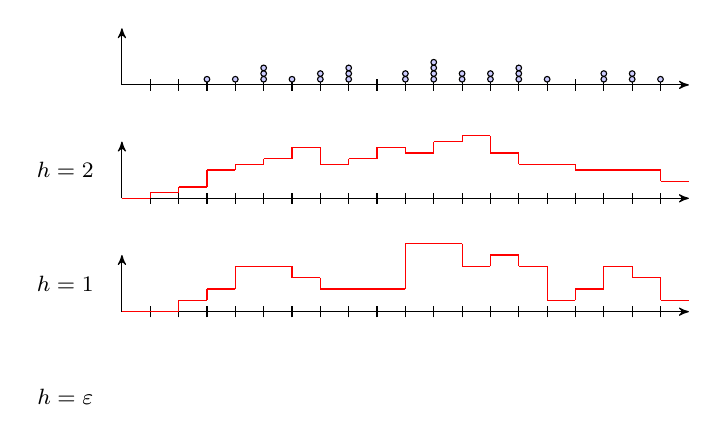
\begin{tikzpicture}[fill=blue!20, every path/.style={draw}, lbl/.style={circle}, scale=0.72]

\draw [->,>=stealth'](-5,8) --(5,8);
\draw [->,>=stealth'](-5,8) --(-5,9);
\draw [-,>=stealth'](-4.5,7.9) --(-4.5,8.1);
\draw [-,>=stealth'](-4,7.9) --(-4,8.1);
\draw [-,>=stealth'](-3.5,7.9) --(-3.5,8.1);
\draw [-,>=stealth'](-3,7.9) --(-3,8.1);
\draw [-,>=stealth'](-2.5,7.9) --(-2.5,8.1);
\draw [-,>=stealth'](-2,7.9) --(-2,8.1);
\draw [-,>=stealth'](-1.5,7.9) --(-1.5,8.1);
\draw [-,>=stealth'](-1,7.9) --(-1,8.1);
\draw [-,>=stealth'](-.5,7.9) --(-.5,8.1);
\draw [-,>=stealth'](0,7.9) --(0,8.1);
\draw [-,>=stealth'](4.5,7.9) --(4.5,8.1);
\draw [-,>=stealth'](4,7.9) --(4,8.1);
\draw [-,>=stealth'](3.5,7.9) --(3.5,8.1);
\draw [-,>=stealth'](3,7.9) --(3,8.1);
\draw [-,>=stealth'](2.5,7.9) --(2.5,8.1);
\draw [-,>=stealth'](2,7.9) --(2,8.1);
\draw [-,>=stealth'](1.5,7.9) --(1.5,8.1);
\draw [-,>=stealth'](1,7.9) --(1,8.1);
\draw [-,>=stealth'](.5,7.9) --(.5,8.1);

\fill (-3.5,8.1) circle(.05);
\fill (-3,8.1) circle(.05);
\fill (-2.5,8.2) circle(.05);
\fill (-2.5,8.3) circle(.05);
\fill (-2.5,8.1) circle(.05);
\fill (-2,8.1) circle(.05);
\fill (-1.5,8.1) circle(.05);
\fill (-1.5,8.2) circle(.05);
\fill (-1,8.1) circle(.05);
\fill (-1,8.2) circle(.05);
\fill (-1,8.3) circle(.05);
\fill (0,8.1) circle(.05);
\fill (0,8.2) circle(.05);
\fill (.5,8.1) circle(.05);
\fill (.5,8.2) circle(.05);
\fill (.5,8.3) circle(.05);
\fill (.5,8.4) circle(.05);
\fill (1,8.1) circle(.05);
\fill (1,8.2) circle(.05);
\fill (1.5,8.1) circle(.05);
\fill (1.5,8.2) circle(.05);
\fill (2,8.1) circle(.05);
\fill (2,8.2) circle(.05);
\fill (2,8.3) circle(.05);
\fill (2.5,8.1) circle(.05);
\fill (3.5,8.1) circle(.05);
\fill (3.5,8.2) circle(.05);
\fill (4,8.1) circle(.05);
\fill (4,8.2) circle(.05);
\fill (4.5,8.1) circle(.05);

\draw [->,>=stealth'](-5,6) --(5,6);
\draw [->,>=stealth'](-5,6) --(-5,7);
\draw [-,>=stealth'](-4.5,5.9) --(-4.5,6.1);
\draw [-,>=stealth'](-4,5.9) --(-4,6.1);
\draw [-,>=stealth'](-3.5,5.9) --(-3.5,6.1);
\draw [-,>=stealth'](-3,5.9) --(-3,6.1);
\draw [-,>=stealth'](-2.5,5.9) --(-2.5,6.1);
\draw [-,>=stealth'](-2,5.9) --(-2,6.1);
\draw [-,>=stealth'](-1.5,5.9) --(-1.5,6.1);
\draw [-,>=stealth'](-1,5.9) --(-1,6.1);
\draw [-,>=stealth'](-.5,5.9) --(-.5,6.1);
\draw [-,>=stealth'](0,5.9) --(0,6.1);
\draw [-,>=stealth'](4.5,5.9) --(4.5,6.1);
\draw [-,>=stealth'](4,5.9) --(4,6.1);
\draw [-,>=stealth'](3.5,5.9) --(3.5,6.1);
\draw [-,>=stealth'](3,5.9) --(3,6.1);
\draw [-,>=stealth'](2.5,5.9) --(2.5,6.1);
\draw [-,>=stealth'](2,5.9) --(2,6.1);
\draw [-,>=stealth'](1.5,5.9) --(1.5,6.1);
\draw [-,>=stealth'](1,5.9) --(1,6.1);
\draw [-,>=stealth'](.5,5.9) --(.5,6.1);

\draw [red, -,>=stealth'](-5,6) --(-4.5,6);
\draw [red, -,>=stealth'](-4.5,6) --(-4.5,6.1);
\draw [red, -,>=stealth'](-4.5,6.1) --(-4,6.1);
\draw [red, -,>=stealth'](-4,6.1) --(-4,6.2);
\draw [red, -,>=stealth'](-4,6.2) --(-3.5,6.2);
\draw [red, -,>=stealth'](-3.5,6.2) --(-3.5,6.5);
\draw [red, -,>=stealth'](-3.5,6.5) --(-3,6.5);
\draw [red, -,>=stealth'](-3,6.5) --(-3,6.6);
\draw [red, -,>=stealth'](-3,6.6) --(-2.5,6.6);
\draw [red, -,>=stealth'](-2.5,6.6) --(-2.5,6.7);
\draw [red, -,>=stealth'](-2.5,6.7) --(-2,6.7);
\draw [red, -,>=stealth'](-2,6.7) --(-2,6.9);
\draw [red, -,>=stealth'](-2,6.9) --(-1.5,6.9);
\draw [red, -,>=stealth'](-1.5,6.9) --(-1.5,6.6);
\draw [red, -,>=stealth'](-1.5,6.6) --(-1,6.6);
\draw [red, -,>=stealth'](-1,6.6) --(-1,6.7);
\draw [red, -,>=stealth'](-1,6.7) --(-.5,6.7);
\draw [red, -,>=stealth'](-.5,6.7) --(-.5,6.9);
\draw [red, -,>=stealth'](-.5,6.9) --(0,6.9);
\draw [red, -,>=stealth'](0,6.9) --(0,6.8);
\draw [red, -,>=stealth'](0,6.8) --(.5,6.8);
\draw [red, -,>=stealth'](.5,6.8) --(.5,7);
\draw [red, -,>=stealth'](.5,7) --(1,7);
\draw [red, -,>=stealth'](1,7) --(1,7.1);
\draw [red, -,>=stealth'](1,7.1) --(1.5,7.1);
\draw [red, -,>=stealth'](1.5,7.1) --(1.5,6.8);
\draw [red, -,>=stealth'](1.5,6.8) --(2,6.8);
\draw [red, -,>=stealth'](2,6.8) --(2,6.6);
\draw [red, -,>=stealth'](2,6.6) --(2.5,6.6);
\draw [red, -,>=stealth'](2.5,6.6) --(3,6.6);
\draw [red, -,>=stealth'](3,6.6) --(3,6.5);
\draw [red, -,>=stealth'](3,6.5) --(3.5,6.5);
\draw [red, -,>=stealth'](3.5,6.5) --(4.5,6.5);
\draw [red, -,>=stealth'](4.5,6.5) --(4.5,6.3);
\draw [red, -,>=stealth'](4.5,6.3) --(5,6.3);

\draw [->,>=stealth'](-5,4) --(5,4);
\draw [->,>=stealth'](-5,4) --(-5,5);
\draw [-,>=stealth'](-4.5,3.9) --(-4.5,4.1);
\draw [-,>=stealth'](-4,3.9) --(-4,4.1);
\draw [-,>=stealth'](-3.5,3.9) --(-3.5,4.1);
\draw [-,>=stealth'](-3,3.9) --(-3,4.1);
\draw [-,>=stealth'](-2.5,3.9) --(-2.5,4.1);
\draw [-,>=stealth'](-2,3.9) --(-2,4.1);
\draw [-,>=stealth'](-1.5,3.9) --(-1.5,4.1);
\draw [-,>=stealth'](-1,3.9) --(-1,4.1);
\draw [-,>=stealth'](-.5,3.9) --(-.5,4.1);
\draw [-,>=stealth'](0,3.9) --(0,4.1);
\draw [-,>=stealth'](4.5,3.9) --(4.5,4.1);
\draw [-,>=stealth'](4,3.9) --(4,4.1);
\draw [-,>=stealth'](3.5,3.9) --(3.5,4.1);
\draw [-,>=stealth'](3,3.9) --(3,4.1);
\draw [-,>=stealth'](2.5,3.9) --(2.5,4.1);
\draw [-,>=stealth'](2,3.9) --(2,4.1);
\draw [-,>=stealth'](1.5,3.9) --(1.5,4.1);
\draw [-,>=stealth'](1,3.9) --(1,4.1);
\draw [-,>=stealth'](.5,3.9) --(.5,4.1);

\draw [red, -,>=stealth'](-5,4) --(-4,4);
\draw [red, -,>=stealth'](-4,4) --(-4,4.2);
\draw [red, -,>=stealth'](-4,4.2) --(-3.5,4.2);
\draw [red, -,>=stealth'](-3.5,4.2) --(-3.5,4.4);
\draw [red, -,>=stealth'](-3.5,4.4) --(-3,4.4);
\draw [red, -,>=stealth'](-3,4.4) --(-3,4.8);
\draw [red, -,>=stealth'](-3,4.8) --(-2,4.8);
\draw [red, -,>=stealth'](-2,4.8) --(-2,4.6);
\draw [red, -,>=stealth'](-2,4.6) --(-1.5,4.6);
\draw [red, -,>=stealth'](-1.5,4.6) --(-1.5,4.4);
\draw [red, -,>=stealth'](-1.5,4.4) --(-.5,4.4);
\draw [red, -,>=stealth'](-.5,4.4) --(0,4.4);
\draw [red, -,>=stealth'](0,4.4) --(0,5.2);
\draw [red, -,>=stealth'](0,5.2) --(1,5.2);
\draw [red, -,>=stealth'](1,5.2) --(1,4.8);
\draw [red, -,>=stealth'](1,4.8) --(1.5,4.8);
\draw [red, -,>=stealth'](1.5,4.8) --(1.5,5);
\draw [red, -,>=stealth'](1.5,5) --(2,5);
\draw [red, -,>=stealth'](2,5) --(2,4.8);
\draw [red, -,>=stealth'](2,4.8) --(2.5,4.8);
\draw [red, -,>=stealth'](2.5,4.8) --(2.5,4.2);
\draw [red, -,>=stealth'](2.5,4.2) --(3,4.2);
\draw [red, -,>=stealth'](3,4.2) --(3,4.4);
\draw [red, -,>=stealth'](3,4.4) --(3.5,4.4);
\draw [red, -,>=stealth'](3.5,4.4) --(3.5,4.8);
\draw [red, -,>=stealth'](3.5,4.8) --(4,4.8);
\draw [red, -,>=stealth'](4,4.8) --(4,4.6);
\draw [red, -,>=stealth'](4,4.6) --(4.5,4.6);
\draw [red, -,>=stealth'](4.5,4.6) --(4.5,4.2);
\draw [red, -,>=stealth'](4.5,4.2) --(5,4.2);

\draw(-6,2.5) node {\footnotesize $h=\varepsilon$};
\draw(-6,4.5) node {\footnotesize $h=1$};
\draw(-6,6.5) node {\footnotesize $h=2$};
\end{tikzpicture}
  \end{center}
  \begin{center}
    \small Effect of bandwidth $h$ on the histogram density estimate: from rough ($h=\varepsilon$) to oversmoothed ($h=2$).
  \end{center}
\end{frame}

\begin{frame}{The Bias--Variance Trade-off in Bandwidth Selection}
  \begin{itemize}
    \item The bandwidth effect illustrates a \alert{key principle} that reappears throughout nonparametric learning.
  \end{itemize}
  \vspace{0.4em}
  \begin{columns}[t]
    \column{0.48\textwidth}
      \begin{alertblock}{$h$ too large}
        The estimate is \textbf{overly smooth} and may wash out important structure.\\
        $\Rightarrow$ \textbf{High bias}.
      \end{alertblock}
    \column{0.48\textwidth}
      \begin{alertblock}{$h$ too small}
        The estimate follows random fluctuations of the sample.\\
        $\Rightarrow$ \textbf{High variance}.
      \end{alertblock}
  \end{columns}
  \vspace{0.5em}
  \begin{block}{Goal}
    Selecting $h$ amounts to choosing a compromise between these two sources of error.
  \end{block}
\end{frame}

\begin{frame}{Smooth Kernels: Beyond the Histogram}
  \begin{itemize}
    \item The hypercube kernel weights all points inside the region equally.
    \item \alert{Smooth kernels} give higher weight to samples close to $\x$ and lower weight to samples farther away.
    \item This produces \textbf{continuous density estimates} and often better practical behavior.
    \item A family of kernels $\kappa_h(\u)$ parameterized by bandwidth $h > 0$:
  \end{itemize}
  \vspace{0.3em}
  \begin{block}{Valid Kernel Conditions}
    \[
      \int \kappa_h(\u)\,d\u = 1, \qquad
      \mathbb{E}[\u] = \mathbf{0}, \qquad
      \mathbb{E}[\u^2] > 0.
    \]
  \end{block}
\end{frame}

\begin{frame}{The General Parzen Window Estimate with Smooth Kernels}
  \begin{itemize}
    \item With a smooth kernel, the Parzen window estimate takes the compact form:
  \end{itemize}
  \begin{block}{Smooth Parzen Window Estimator}
    \[
      p(\x) = \frac{1}{n}\sum_{i=1}^{n}\kappa_h(\x-\x_i).
    \]
  \end{block}
  \vspace{0.4em}
  \begin{itemize}
    \item Interpretation: place around each sample $\x_i$ a small ``bump'' of mass $1/n$ and sum them up.
    \item The bandwidth $h$ controls the \alert{width} of each bump.
  \end{itemize}
\end{frame}

\begin{frame}{Common Kernels}
  \begin{block}{Gaussian Kernel}
    Infinitely smooth, infinite support:
    \[
      \kappa_h(\u) = \frac{1}{(\sqrt{2\pi}h)^d}\exp\!\left(-\frac{\|\u\|^2}{2h^2}\right).
    \]
  \end{block}
  \vspace{0.4em}
  \begin{block}{Epanechnikov Kernel}
    Compact support, computationally efficient:
    \[
      \kappa_h(\u) = \frac{3}{4h}\left(1 - \frac{\u^2}{h^2}\right)\quad\text{for }|\u| \le h,
      \qquad
      \kappa_h(\u) = 0\text{ otherwise.}
    \]
  \end{block}
  \vspace{0.2em}
  \begin{itemize}
    \item Although different, the \alert{role of $h$} remains the same in both: it controls the locality and therefore the bias--variance trade-off.
  \end{itemize}
\end{frame}

\begin{frame}{Figure: Comparison of Kernel Functions}
  \begin{center}
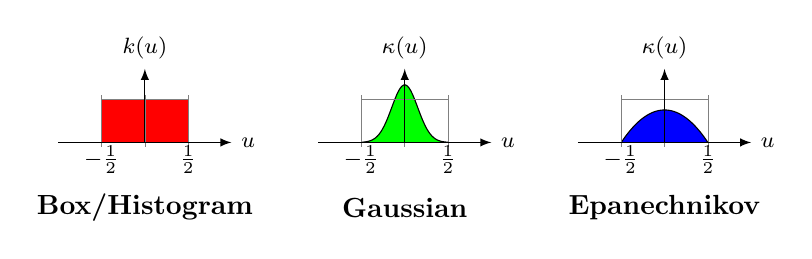
\begin{tikzpicture}[scale=0.55]

% Box kernel
\begin{scope}[xshift=-6cm]
\fill[color=red, samples=50] plot (-1,0)--(-1,1)--(1,1)--(1,0)--cycle;
\draw[color=black, samples=50] (-1,0)--(-1,1)--(1,1)--(1,0);
\draw[very thin,color=gray] (-1,-0.1) grid (1,1.1);
\draw[->] (-2,0) -- (2,0) node[right] {\footnotesize $u$};
\draw[->] (0,0) -- (0,1.7) node[above] {\footnotesize $k(u)$};
\draw(1,-0.4) node {\footnotesize $\frac{1}{2}$};
\draw(-1,-0.4) node {\footnotesize $-\frac{1}{2}$};
\node at (0,-1.5) {\textbf{Box/Histogram}};
\end{scope}

% Gaussian kernel
\begin{scope}[xshift=0cm]
\fill[color=green, samples=50] plot[domain=-1:1] (\x,{1/(.3*sqrt(2*3.14159))*exp(-(\x*\x)/(2*.09))})--cycle;
\draw[color=black, samples=50, domain=-1:1] plot (\x,{1/(.3*sqrt(2*3.14159))*exp(-(\x*\x)/(2*.09))});
\draw[very thin,color=gray] (-1,-0.1) grid (1,1.1);
\draw[->] (-2,0) -- (2,0) node[right] {\footnotesize $u$};
\draw[->] (0,0) -- (0,1.7) node[above] {\footnotesize $\kappa(u)$};
\draw(1,-0.4) node {\footnotesize $\frac{1}{2}$};
\draw(-1,-0.4) node {\footnotesize $-\frac{1}{2}$};
\node at (0,-1.5) {\textbf{Gaussian}};
\end{scope}

% Epanechnikov kernel
\begin{scope}[xshift=6cm]
\fill[color=blue, samples=50, domain=-1:1] plot (\x,{3/4*(1-\x*\x)})--cycle;
\draw[color=black, samples=50, domain=-1:1] plot (\x,{3/4*(1-\x*\x)});
\draw[very thin,color=gray] (-1,-0.1) grid (1,1.1);
\draw[->] (-2,0) -- (2,0) node[right] {\footnotesize $u$};
\draw[->] (0,0) -- (0,1.7) node[above] {\footnotesize $\kappa(u)$};
\draw(1,-0.4) node {\footnotesize $\frac{1}{2}$};
\draw(-1,-0.4) node {\footnotesize $-\frac{1}{2}$};
\node at (0,-1.5) {\textbf{Epanechnikov}};
\end{scope}

\end{tikzpicture}
  \end{center}
  \begin{center}
    \small Common kernel functions for Parzen window density estimation.
  \end{center}
\end{frame}

%% ════════════════════════════════════════════════════════════════════════════
\section{Bandwidth Selection}

\begin{frame}{Bandwidth Selection: The Central Hyperparameter}
  \begin{itemize}
    \item The bandwidth $h$ is the \alert{central hyperparameter} of kernel density estimation.
    \item Too large $\Rightarrow$ biased estimator; too small $\Rightarrow$ unstable estimator.
    \item Two main strategies: \textbf{heuristic rules} and \textbf{data-driven criteria}.
  \end{itemize}
  \vspace{0.5em}
  \begin{block}{Rule of Thumb (Silverman)}
    Motivated by optimality under Gaussian assumptions:
    \[
      h^* = 1.06\,\hat{\sigma}\,n^{-1/5},
    \]
    where $\hat{\sigma}$ is the sample standard deviation.
  \end{block}
\end{frame}

\begin{frame}{Cross-Validation for Bandwidth Selection}
  \begin{itemize}
    \item A more principled approach: choose $h$ by \alert{cross-validation}.
    \item A common criterion maximizes the \textbf{leave-one-out log-likelihood}:
  \end{itemize}
  \begin{block}{Leave-One-Out Log-Likelihood}
    \[
      h^* = \argmax{h}\; \frac{1}{n}\sum_{i=1}^{n} \log p_{-i}(\x_i),
    \]
    where $p_{-i}(\x_i)$ is the density estimate at $\x_i$ computed using all samples except $\x_i$.
  \end{block}
  \vspace{0.3em}
  \begin{itemize}
    \item This criterion directly measures how well the estimated density \alert{predicts unseen data points}.
  \end{itemize}
\end{frame}

%% ════════════════════════════════════════════════════════════════════════════
\section{Classification via KDE}

\begin{frame}{KDE as a Classification Method}
  \begin{itemize}
    \item Kernel density estimation becomes a \alert{classification method} when applied class-wise.
    \item For each class $C_i$, collect the training points belonging to that class and build a class-conditional density estimate:
    \[
      p(\x \mid C_i) = \frac{1}{n_i}\sum_{j:\,t_j=i}\kappa_h(\x-\x_j),
    \]
    where $n_i$ is the number of training samples in class $C_i$.
    \item The class prior is estimated empirically:
    \[
      p(C_i) = \frac{n_i}{n}.
    \]
  \end{itemize}
\end{frame}

\begin{frame}{KDE Classification Decision Rule}
  \begin{itemize}
    \item Bayes' rule yields a posterior proportional to $p(\x \mid C_i)\,p(C_i)$.
  \end{itemize}
  \begin{block}{KDE Classifier}
    \[
      \hat{C} = \argmax{i}\; p(\x \mid C_i)\,p(C_i).
    \]
  \end{block}
  \vspace{0.5em}
  \begin{itemize}
    \item This is a \alert{nonparametric analogue} of generative classification.
    \item Instead of assuming a parametric form for $p(\x \mid C_i)$, it is estimated directly from data.
    \item A single bandwidth $h$ controls all class-conditional density estimates.
  \end{itemize}
\end{frame}

%% ════════════════════════════════════════════════════════════════════════════
\section{$k$-Nearest Neighbors Classification}

\begin{frame}{The $k$-NN Principle}
  \framesubtitle{Fixed $k$, variable volume}
  \begin{itemize}
    \item $k$-NN starts from the same identity $p(\x) \approx k/(nV)$ but enforces locality differently.
    \item Fix the number of neighbors $k$ and let the region \alert{expand} until it contains exactly $k$ samples.
    \item Let $r_k(\x)$ be the distance from $\x$ to its $k$-th nearest neighbor.
    \item Using a $d$-dimensional ball of radius $r_k(\x)$:
    \[
      V = c_d\,r_k(\x)^d,
    \]
    where $c_d$ is the volume of the unit $d$-dimensional ball.
  \end{itemize}
\end{frame}

\begin{frame}{$k$-NN Density Estimate}
  \begin{block}{$k$-NN Density Estimator}
    \[
      p(\x) \approx \frac{k}{n \cdot c_d \cdot r_k(\x)^d}.
    \]
  \end{block}
  \vspace{0.5em}
  \begin{itemize}
    \item This expression makes explicit how density is \alert{inversely related to the radius} needed to capture $k$ points.
    \item Where data are dense: $r_k(\x)$ is \textbf{small} $\Rightarrow$ estimated density is \textbf{high}.
    \item Where data are sparse: $r_k(\x)$ is \textbf{large} $\Rightarrow$ estimated density is \textbf{low}.
    \item The neighborhood \alert{automatically adapts} to local data density.
  \end{itemize}
\end{frame}

\begin{frame}{$k$-NN Classification: Probabilistic Motivation}
  \begin{itemize}
    \item For classification, approximate class-conditional densities within the local region:
    \[
      p(\x \mid C_i) = \frac{k_i}{n_i V}, \qquad p(\x) = \frac{k}{nV}.
    \]
    \item Substituting into Bayes' rule with $p(C_i) = n_i/n$:
  \end{itemize}
  \begin{block}{Posterior from Local Counts}
    \[
      p(C_i \mid \x)
      = \frac{p(\x \mid C_i)\,p(C_i)}{p(\x)}
      = \frac{\dfrac{k_i}{n_i V} \cdot \dfrac{n_i}{n}}{\dfrac{k}{nV}}
      = \frac{k_i}{k}.
    \]
  \end{block}
  \vspace{0.2em}
  \begin{itemize}
    \item The posterior is simply the \alert{fraction of neighbors in each class}.
  \end{itemize}
\end{frame}

\begin{frame}{$k$-NN Decision Rule: Majority Voting}
  \begin{itemize}
    \item Since $p(C_i \mid \x) = k_i/k$, the maximum-posterior decision rule reduces to:
  \end{itemize}
  \begin{block}{$k$-NN Classifier}
    \[
      \hat{C} = \argmax{i}\; k_i,
    \]
    i.e., \alert{majority vote} among the $k$ nearest neighbors.
  \end{block}
  \vspace{0.5em}
  \begin{itemize}
    \item The remarkable simplicity of this rule is one reason $k$-NN is frequently used as a \textbf{baseline method}.
    \item No explicit density estimate is needed.
    \item The rule is completely non-parametric: no assumptions on the form of $p(\x \mid C_i)$.
  \end{itemize}
\end{frame}

\begin{frame}{Effect of $k$ on Decision Boundaries}
  \begin{itemize}
    \item The value of $k$ controls the \alert{smoothness} of the resulting decision boundary.
  \end{itemize}
  \vspace{0.3em}
  \begin{columns}[t]
    \column{0.48\textwidth}
      \begin{alertblock}{Small $k$}
        Highly flexible boundaries that can track individual training samples.\\
        Risk: \textbf{overfitting}.
      \end{alertblock}
    \column{0.48\textwidth}
      \begin{block}{Large $k$}
        Smoother boundaries that average over more samples.\\
        Risk: \textbf{underfitting}.
      \end{block}
  \end{columns}
\end{frame}

\begin{frame}{Figure: $k$-NN Decision Boundaries ($k=1$)}
  \begin{center}
    
\includegraphics[width=0.25\textwidth]{figs/Figure2-28a.pdf}
  \end{center}
  \begin{center}
    \small $k$-NN decision boundary for $k=1$: highly irregular, fits individual training points.
  \end{center}
\end{frame}

\begin{frame}{Figure: $k$-NN Decision Boundaries ($k=$ moderate)}
  \begin{center}
    
\includegraphics[width=0.25\textwidth]{figs/Figure2-28b.pdf}
  \end{center}
  \begin{center}
    \small $k$-NN decision boundary for a moderate value of $k$: smoother regions emerge.
  \end{center}
\end{frame}

\begin{frame}{Figure: $k$-NN Decision Boundaries ($k=$ large)}
  \begin{center}
    
\includegraphics[width=0.25\textwidth]{figs/Figure2-28c.pdf}
  \end{center}
  \begin{center}
    \small $k$-NN decision boundary for large $k$: very smooth boundary, may underfit.
  \end{center}
\end{frame}

%% ════════════════════════════════════════════════════════════════════════════
\section{Theoretical Properties and Practical Considerations}

\begin{frame}{Asymptotic Properties of $k$-NN}
  \begin{block}{Consistency}
    With appropriate choices of $k = k(n)$ as $n \to \infty$, the $k$-NN method is \alert{consistent} and approaches the \textbf{Bayes optimal error rate}.
  \end{block}
  \vspace{0.5em}
  \begin{itemize}
    \item Theoretical guarantees exist, but finite-sample behavior depends strongly on design choices.
    \item The most important design choice: the value of $k$.
  \end{itemize}
\end{frame}

\begin{frame}{Choosing $k$}
  \begin{itemize}
    \item \textbf{$k=1$}: extremely local classifier; every training point becomes a ``prototype''.
      \begin{itemize}
        \item Highly flexible but prone to \alert{overfitting}.
        \item Sensitive to noise and outliers.
      \end{itemize}
    \item \textbf{Large $k$}: predictions average over more samples; more stable but boundary becomes too smooth.
    \item \textbf{Practical heuristic}: $k \approx \sqrt{n}$.
    \item \textbf{Best practice}: choose $k$ by \alert{cross-validation}, keeping in mind that the optimal value depends on noise level, class overlap, and dimension.
  \end{itemize}
\end{frame}

\begin{frame}{The Distance Metric}
  \begin{itemize}
    \item Nearest-neighbor methods rely \alert{entirely} on the notion of distance.
    \item Feature scaling and metric selection can \alert{dramatically affect} performance.
  \end{itemize}
  \vspace{0.4em}
  \begin{block}{Common Distance Metrics}
    \begin{itemize}
      \item \textbf{Euclidean}: $\|\x - \x'\|_2$ — standard, isotropic.
      \item \textbf{Manhattan}: $\|\x - \x'\|_1$ — robust to outliers in individual features.
      \item \textbf{Mahalanobis}: accounts for correlations and scales in the data.
      \item \textbf{Cosine distance}: suitable for high-dimensional, sparse data.
    \end{itemize}
  \end{block}
\end{frame}

\begin{frame}{The Curse of Dimensionality}
  \begin{alertblock}{A Key Challenge}
    In high-dimensional spaces, distances tend to \alert{concentrate}: all points become approximately equidistant, weakening the notion of ``nearest neighbor.''
  \end{alertblock}
  \vspace{0.4em}
  \begin{itemize}
    \item The volume of the hypersphere capturing $k$ neighbors grows exponentially with dimension.
    \item A local neighborhood in high dimensions may need to cover a substantial fraction of the feature space.
    \item Performance can degrade significantly as dimensionality increases.
    \item Mitigation: feature selection, dimensionality reduction, metric learning.
  \end{itemize}
\end{frame}

\begin{frame}{Computational Aspects: Lazy Learning}
  \begin{itemize}
    \item $k$-NN is often described as a \alert{lazy} learning method.
    \item \textbf{Training}: minimal computation — essentially just storing the dataset.
    \item \textbf{Prediction}: most effort deferred to query time, requiring a nearest-neighbor search.
  \end{itemize}
  \vspace{0.4em}
  \begin{block}{Search Complexity}
    \begin{itemize}
      \item Naive search: $O(n)$ per query (compare to every training point).
      \item Acceleration structures (KD-trees, ball trees): reduce cost for low to moderate dimensions.
      \item Benefits of acceleration \alert{diminish as dimensionality increases}.
    \end{itemize}
  \end{block}
\end{frame}

%% ════════════════════════════════════════════════════════════════════════════
\section{KDE vs.\ $k$-NN: A Comparison}

\begin{frame}{KDE vs.\ $k$-NN: Two Sides of the Same Principle}
  \begin{itemize}
    \item Both KDE and $k$-NN implement a \alert{local counting principle}, starting from $p(\x) \approx k/(nV)$.
  \end{itemize}
  \vspace{0.4em}
  \begin{columns}[t]
    \column{0.48\textwidth}
      \begin{block}{KDE}
        \begin{itemize}
          \item \textbf{Fix}: volume $V$ (via bandwidth $h$).
          \item \textbf{Vary}: number of points $k$.
          \item Yields smooth density estimates by construction.
          \item Natural when a scale $h$ is known.
        \end{itemize}
      \end{block}
    \column{0.48\textwidth}
      \begin{block}{$k$-NN}
        \begin{itemize}
          \item \textbf{Fix}: number of points $k$.
          \item \textbf{Vary}: volume $V$.
          \item Automatically adapts neighborhood to local data density.
          \item Advantageous in heterogeneous datasets.
        \end{itemize}
      \end{block}
  \end{columns}
\end{frame}

\begin{frame}{Practical Trade-offs}
  \begin{itemize}
    \item \textbf{KDE}: convenient when a natural scale $h$ is known or can be tuned; prediction can be smooth for small $k$ but requires evaluating all training kernels.
    \item \textbf{$k$-NN}: the prediction rule can be less smooth for small $k$; but the majority vote rule is intuitive and requires no density evaluation.
    \item Both approaches can be sensitive to the choice of their respective hyperparameters ($h$ vs.\ $k$).
    \item The \alert{curse of dimensionality} affects both equally.
  \end{itemize}
\end{frame}

%% ════════════════════════════════════════════════════════════════════════════
\section{Summary}

\begin{frame}{Summary: Key Formulas}
  \renewcommand{\arraystretch}{1.5}
  \begin{center}
  \begin{tabular}{ll}
    \toprule
    \textbf{Result} & \textbf{Formula} \\
    \midrule
    Local density estimate & $p(\x) \approx k/(nV)$ \\
    Parzen (hypercube) & $p_n(\x) = \frac{1}{nh^d}\sum_{i=1}^n k\!\left(\frac{\x-\x_i}{h}\right)$ \\
    Parzen (smooth) & $p(\x) = \frac{1}{n}\sum_{i=1}^n \kappa_h(\x - \x_i)$ \\
    Silverman rule & $h^* = 1.06\,\hat{\sigma}\,n^{-1/5}$ \\
    LOO bandwidth & $h^* = \argmax{h}\frac{1}{n}\sum_i \log p_{-i}(\x_i)$ \\
    $k$-NN density & $p(\x) \approx k/(n\cdot c_d\cdot r_k(\x)^d)$ \\
    $k$-NN posterior & $p(C_i \mid \x) = k_i/k$ \\
    $k$-NN decision & $\hat{C} = \argmax{i}\; k_i$ \\
    KDE classifier & $\hat{C} = \argmax{i}\; p(\x \mid C_i)\,p(C_i)$ \\
    \bottomrule
  \end{tabular}
  \end{center}
\end{frame}

\begin{frame}{Summary: Methods at a Glance}
  \begin{columns}[t]
    \column{0.48\textwidth}
      \begin{block}{Kernel Density Estimation}
        \begin{itemize}
          \item Fix volume via bandwidth $h$.
          \item Parzen window: sum of bumps.
          \item Gaussian or Epanechnikov kernels.
          \item Tune $h$ via rule of thumb or cross-validation.
          \item Apply class-wise for classification.
        \end{itemize}
      \end{block}
    \column{0.48\textwidth}
      \begin{block}{$k$-Nearest Neighbors}
        \begin{itemize}
          \item Fix $k$, let volume vary.
          \item Posterior $= k_i/k$ (majority vote).
          \item Tune $k$ by cross-validation.
          \item Lazy learning: fast training, slow prediction.
          \item Consistent asymptotically.
        \end{itemize}
      \end{block}
  \end{columns}
  \vspace{0.5em}
  \begin{alertblock}{Common Challenges}
    Both methods suffer from the curse of dimensionality and require careful hyperparameter tuning.
  \end{alertblock}
\end{frame}

\begin{frame}{Nonparametric Methods in Context}
  \begin{itemize}
    \item Nonparametric methods are \alert{canonical tools} in density estimation and classification.
    \item Both KDE and $k$-NN implement a locality principle through neighborhoods around query points.
    \item Both become more expressive as the dataset grows.
  \end{itemize}
  \vspace{0.4em}
  \begin{block}{Strengths}
    Flexibility, minimal assumptions, consistency under suitable conditions.
  \end{block}
  \vspace{0.3em}
  \begin{alertblock}{Limitations}
    Computational cost; curse of dimensionality; naive locality assumptions can be ineffective in high-dimensional spaces.
  \end{alertblock}
  \vspace{0.3em}
  \begin{itemize}
    \item Despite challenges, they remain valuable as \textbf{baselines}, as \textbf{conceptual tools}, and as \textbf{building blocks} for modern algorithms.
  \end{itemize}
\end{frame}

%\end{document}
